\begin{abox}
	Practise Set-1
\end{abox}
\begin{enumerate}[label=\color{ocre}\textbf{\arabic*.}]
	\item The value of the integral $\int_{C} d z z^{2} e^{z}$, where $C$ is an open contour in the complex $z$-plane as shown in the figure below, is:
	{\exyear{NET/JRF(JUNE-2011)}}
	\begin{figure}[H]
		\centering
		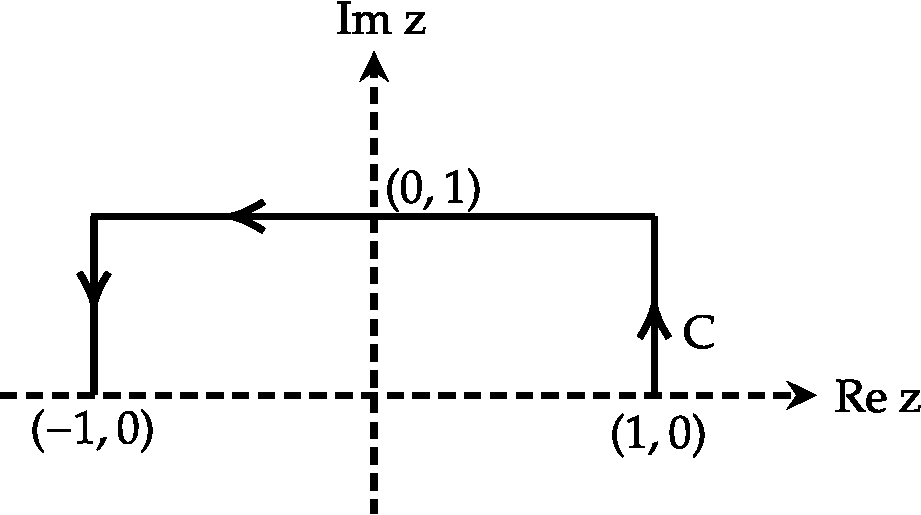
\includegraphics[height=4cm,width=8cm]{diagram-20211005-crop}
	\end{figure}
	\begin{tasks}(4)
		\task[\textbf{A.}] $\frac{5}{e}+e$
		\task[\textbf{B.}] $e-\frac{5}{e}$
		\task[\textbf{C.}] $\frac{5}{e}-e$
		\task[\textbf{D.}] $-\frac{5}{e}-e$
	\end{tasks}
	\begin{answer}
		\begin{align*}
		\intertext { If we complete the contour, then by Cauchy integral theorem }
		\int_{-1}^{1} d z z^{2} e^{z}+\int_{C} d z z^{2} e^{z}&=0 \Rightarrow \int_{C} d z z^{2} e^{z}=-\int_{-1}^{1} d z z^{2} e^{z}\\&=-\left[z^{2} e^{z}-2 z e^{2}+2 e^{2}\right]_{-1}^{1}=\frac{5}{e}-e
		\end{align*}
		So the correct answer is \textbf{Option (C)}
	\end{answer}
	\item Which of the following is an analytic function of the complex variable $z=x+i y$ in the domain $|z|<2 ?$
	{\exyear{NET/JRF(JUNE-2011)}}
	\begin{tasks}(2)
		\task[\textbf{A.}] $(3+x-i y)^{7}$
		\task[\textbf{B.}] $(1+x+i y)^{4}(7-x-i y)^{3}$
		\task[\textbf{C.}] $(1-x-i y)^{4}(7-x+i y)^{3}$
		\task[\textbf{D.}] $(x+i y-1)^{1 / 2}$
	\end{tasks}
	\begin{answer}
		Put $z=x+i y .$ If $\bar{z}=x-i y$ appears in any of the expressions then that expression is non-analytic. For option (D) we have a branch point singularity as the power is $\frac{1}{2}$ which is fractional. Hence only option (B) is analytic.\\\\
		So the correct answer is \textbf{Option (B)}
	\end{answer}
	\item The first few terms in the Laurent series for $\frac{1}{(z-1)(z-2)}$ in the region $1 \leq|z| \leq 2$ and around $z=1$ is
	{\exyear{NET/JRF(JUNE-2012)}}
	\begin{tasks}(1)
		\task[\textbf{A.}] $\frac{1}{2}\left[1+z+z^{2}+\ldots\right]\left[1+\frac{z}{2}+\frac{z^{2}}{4}+\frac{z^{3}}{8}+\ldots .\right]$
		\task[\textbf{B.}] $\frac{1}{1-z}-z-(1-z)^{2}+(1-z)^{3}+\ldots .$
		\task[\textbf{C.}] $\frac{1}{\mathrm{z}^{2}}\left[1+\frac{1}{\mathrm{z}}+\frac{1}{\mathrm{z}^{2}}+\ldots .\right]\left[1+\frac{2}{\mathrm{z}}+\frac{4}{\mathrm{z}^{2}}+\ldots . .\right]$
		\task[\textbf{D.}]  $2(z-1)+5(z-1)^{2}+7(z-1)^{3}+\ldots$
	\end{tasks}
	\begin{answer}
		\begin{align*}
		\frac{1}{(z-1)(z-2)}&=\frac{1}{z-2}-\frac{1}{z-1}=\frac{1}{1-z}+\frac{1}{(z-1)-1}\\&=\frac{1}{1-z}-(1+(1-z))^{-1}\\
		&=\frac{1}{1-z}-\left[1+(1-z)+\frac{(-1)(-2)}{2 !}(1-z)^{2}+\frac{(-1)(-2)(-3)}{3 !}(1-z)^{3} \ldots\right]\\
		&=\frac{1}{1-z}-\left[z+(1-z)^{2}-(1-z)^{3}+\ldots . .\right]
		\end{align*}
		So the correct answer is \textbf{Option (B)}
	\end{answer}
	\item Let $u(x, y)=x+\frac{1}{2}\left(x^{2}-y^{2}\right)$ be the real part of analytic function $f(z)$ of the complex variable $z=x+i y$. The imaginary part of $f(z)$ is
	{\exyear{NET/JRF(JUNE-2012)}}
	\begin{tasks}(4)
		\task[\textbf{A.}] $y+x y$
		\task[\textbf{B.}] $x y$
		\task[\textbf{C.}] $y$
		\task[\textbf{D.}] $y^{2}-x^{2}$
	\end{tasks}
	\begin{answer}
		\begin{align*}
		u(x, y)&=x+\frac{1}{2}\left(x^{2}-y^{2}\right), v(x, y)=?\\
		\text{Check }\frac{\partial u}{\partial x}&=\frac{\partial v}{\partial y}\text{ and } \frac{\partial u}{\partial y}=-\frac{\partial v}{\partial x}\\
		\Rightarrow \frac{\partial u}{\partial x}&=\frac{\partial v}{\partial y}, \quad \frac{\partial v}{\partial y}=1+x, \\ v&=y+x y+f(x)\\
		\frac{\partial u}{\partial y}&=-\frac{\partial v}{\partial x} \Rightarrow \frac{\partial v}{\partial x}=+y, \\ v&=y x+f(y)\\
		y+x y+f(x)&=y x+f(y)\\
		\text{If }f(x)&=0\quad \quad
		f(y)=y\\
		v&=x y+y
		\end{align*}
		So the correct answer is \textbf{Option (A)}
	\end{answer}
	\item The value of the integral $\int_{C} \frac{z^{3} d z}{\left(z^{2}-5 z+6\right)}$, where $C$ is a closed contour defined by the equation $2|z|-5=0$, traversed in the anti-clockwise direction, is
	{\exyear{NET/JRF(DEC-2012)}}
	\begin{tasks}(4)
		\task[\textbf{A.}] $-16 \pi i$
		\task[\textbf{B.}] $16 \pi \mathrm{i}$
		\task[\textbf{C.}] $8 \pi i$
		\task[\textbf{D.}] $2 \pi i$
	\end{tasks}
	\begin{answer}
		\begin{align*}
		z^{2}-5 z+6&=0 \Rightarrow z^{2}-2 z-3 z+6\\&=0 \Rightarrow z(z-2)-3(z-2)=0 \Rightarrow z=3,2\\
		2|z|&=5 \Rightarrow|z|=2.5,\text{ only 2 will be inside.}\\
		\text{Residue }&=\left.(z-2) \frac{z^{3}}{(z-3)(z-2)}\right|_{z=2}=\frac{8}{2-3}\\&=-8 \Rightarrow \int \frac{z^{3} d z}{z^{2}-5 z+6}=2 \pi i(-8)=-16 \pi i
		\end{align*}
		So the correct answer is \textbf{Option (A)}
	\end{answer}
	\item  With $z=x+i y$, which of the following functions $f(x, y)$ is NOT a (complex) analytic function of $z$ ?
	{\exyear{NET/JRF(JUNE-2013)}}
	\begin{tasks}(1)
		\task[\textbf{A.}] $f(x, y)=(x+i y-8)^{3}\left(4+x^{2}-y^{2}+2 i x y\right)^{7}$
		\task[\textbf{B.}] $f(x, y)=(x+i y)^{7}(1-x-i y)^{3}$
		\task[\textbf{C.}] $f(x, y)=\left(x^{2}-y^{2}+2 i x y-3\right)^{5}$
		\task[\textbf{D.}] $f(x, y)=(1-x+i y)^{4}(2+x+i y)^{6}$
	\end{tasks}
	\begin{answer}
		\begin{align*}
		f(x, y)&=(1-x+i y)^{4}(2+x+i y)^{6}\\&=\{1-(x-i y)\}^{4}(2+x+i y)^{6}\\
		\text{Due to present of }\bar{z}&=(x-i y)
		\end{align*}
		So the correct answer is \textbf{Option (D)}
	\end{answer}
	\item  Which of the following functions cannot be the real part of a complex analytic function of $z=x+i y ?$
	{\exyear{NET/JRF(DEC-2013)}}
	\begin{tasks}(4)
		\task[\textbf{A.}] $x^{2} y$
		\task[\textbf{B.}]  $x^{2}-y^{2}$
		\task[\textbf{C.}] $x^{3}-3 x y^{2}$
		\task[\textbf{D.}] $3 x^{2} y-y-y^{3}$
	\end{tasks}
	\begin{answer}
		\begin{align*}
		\intertext{ Let $x^{2} y$ be real part of a complex function. Use Milne Thomson's method to write analytic complex function. The real part of that function should be (1) but that is not the case. So this cannot be real part of an analytic function. Also,}
		z^{2}&=(x+i y)^{2}=x^{2}-y^{2}+2 i x y,\text{ Real part option (2)}\\
		z^{3}&=(x+i y)^{3}=x^{3}-i y^{3}+3 i x y(x+i y)\\
		&=x^{3}-i y^{3}+3 i x^{2} y-3 x y^{2},\text{ Real part option (3)}
		\end{align*}
		So the correct answer is \textbf{Option (A)}
	\end{answer}
	\item  Given that the integral $\int_{0}^{\infty} \frac{d x}{y^{2}+x^{2}}=\frac{\pi}{2 y}$, the value of $\int_{0}^{\infty} \frac{d x}{\left(y^{2}+x^{2}\right)^{2}}$ is
	{\exyear{NET/JRF(DEC-2013)}}
	\begin{tasks}(4)
		\task[\textbf{A.}] $\frac{\pi}{y^{3}}$
		\task[\textbf{B.}] $\frac{\pi}{4 y^{3}}$
		\task[\textbf{C.}]  $\frac{\pi}{8 y^{3}}$
		\task[\textbf{D.}] $\frac{\pi}{2 y^{3}}$
	\end{tasks}
	\begin{answer}
		\begin{align*}
		\int_{0}^{\infty} \frac{d x}{\left(y^{2}+x^{2}\right)^{2}}&=\frac{1}{2} \int_{-\infty}^{\infty} \frac{d x}{\left(y^{2}+x^{2}\right)^{2}},\text{ pole is of }2^{\text {nd }}\text{ order at }x=i y,\text{ residue }=1 /\left(4 i y^{3}\right)\\
		\text{Integral }&=\left(\frac{1}{2}\right)(2 \pi i) \frac{1}{4 i y^{3}}=\frac{\pi}{\left(4 y^{3}\right)}
		\end{align*}
	\end{answer}
	\item If $C$ is the contour defined by $|z|=\frac{1}{2}$, the value of the integral
	$$
	\oint_{C} \frac{d z}{\sin ^{2} z}
	$$
	is
	{\exyear{NET/JRF(JUNE-2014)}}
	\begin{tasks}(4)
		\task[\textbf{A.}] $\infty$
		\task[\textbf{B.}] $2 \pi i$
		\task[\textbf{C.}] 0
		\task[\textbf{D.}] $\pi i$
	\end{tasks}
	\begin{answer}
		\begin{align*}
		f(z)&=\frac{1}{\sin ^{2} z} \quad\left(|z|=\frac{1}{2}\right)\\
		\sin z&=z-\frac{z^{3}}{\lfloor 3}+\frac{z^{5}}{\lfloor 5} \ldots . \Rightarrow \frac{1}{\sin ^{2} z}=\frac{1}{\left(z-\frac{z^{3}}{\frac{3}{3}}+\frac{z^{5}}{5} \cdots\right)^{2}}\\
		\Rightarrow \frac{1}{\sin ^{2} z}&=\frac{1}{z^{2}}\left[1-\frac{z^{2}}{\lfloor 3}+\frac{z^{4}}{\lfloor 5} \ldots .\right]^{-2} \Rightarrow \oint_{C} \frac{d z}{\sin ^{2} z}=0
		\end{align*}
		So the correct answer is \textbf{Option (C)}
	\end{answer}
	\item The principal value of the integral $\int_{-\infty}^{\infty} \frac{\sin (2 x)}{x^{3}} d x$ is
	{\exyear{NET/JRF(DEC-2014)}}
	\begin{tasks}(4)
		\task[\textbf{A.}] $-2 \pi$
		\task[\textbf{B.}]  $-\pi$
		\task[\textbf{C.}] $\pi$
		\task[\textbf{D.}]  $2 \pi$
	\end{tasks}
	\begin{answer}
		\begin{align*}
		\text{Let }f(z)&=\frac{e^{i 2 z}}{z^{3}}\\
		\lim _{2 \rightarrow 0}(z-0)^{3} f(z)&=\lim _{z \rightarrow 0}(z-0)^{3} \frac{e^{i 2 z}}{z^{3}}\\&=1(\text{ finite and }\neq 0) \Rightarrow z=0 \text{is pole of order 3} .\\
		\text{Residue }R&=\frac{1}{2 !} \lim _{z \rightarrow 0} \frac{d^{2}}{d z^{2}}\left[(z-0)^{3} \frac{e^{i 2 z}}{z^{3}}\right]=-2\\
		\Rightarrow \int_{-\infty}^{\infty} f(x) d x&=\pi i \Sigma R=\pi i(-2)=-2 \pi i \Rightarrow \operatorname{Im} .\text{ Part }\\&=-2 \pi \Rightarrow \int_{-\infty}^{\infty} f(x) d x=-2 \pi
		\end{align*}
		So the correct answer is \textbf{Option (A)}
	\end{answer}
	\item The Laurent series expansion of the function $f(z)=e^{2}+e^{1 / 2}$ about $z=0$ is given by
	{\exyear{NET/JRF(DEC-2014)}}
	\begin{tasks}(2)
		\task[\textbf{A.}] $\sum_{n=-\infty}^{\infty} \frac{z^{n}}{n !}$ for all $|z|<\infty$
		\task[\textbf{B.}] $\sum_{n=0}^{\infty}\left(z^{n}+\frac{1}{z^{n}}\right) \frac{1}{n !}$ only if $0<|z|<1$
		\task[\textbf{C.}] $\sum_{n=0}^{\infty}\left(z^{n}+\frac{1}{z^{n}}\right) \frac{1}{n !}$ for all $0<|z|<\infty$
		\task[\textbf{D.}]  $\sum_{n=-\infty}^{\infty} \frac{z^{n}}{n !}$ only if $|z|<1$
	\end{tasks}
	\begin{answer}
		\begin{align*}
		e^{z}&=\left(1+z+\frac{z^{2}}{2 !}+\ldots\right)=\sum_{n=0}^{\infty} \frac{z^{n}}{n !}\text{ and }e^{1 / z}\\&=1+\frac{1}{z}+\frac{1}{2 !} \frac{1}{z^{2}}+\ldots .=\sum_{n=0}^{\infty} \frac{1}{z^{n} n !}\\
		\Rightarrow f(z)&=\left(e^{z}+e^{1 / 2}\right)=\sum_{n=0}^{\infty}\left(z^{n}+\frac{1}{z^{n}}\right) \frac{1}{n !},\text{ for all }0<|z|<\infty
		\end{align*}
		So the correct answer is \textbf{Option (C)}
	\end{answer}
	\item Consider the function $f(z)=\frac{1}{z} \ln (1-z)$ of a complex variable $z=r e^{i \theta}(r \geq 0, \quad-\infty<\theta<\infty)$. The singularities of $f(z)$ are as follows:
	{\exyear{NET/JRF(DEC-2014)}}
	\begin{tasks}(1)
		\task[\textbf{A.}]  Branch points at $z=1$ and $z=\infty$; and a pole at $z=0$ only for $0 \leq \theta<2 \pi$
		\task[\textbf{B.}] Branch points at $z=1$ and $z=\infty$; and a pole at $z=0$ for all $\theta$ other than $0 \leq \theta<2 \pi$
		\task[\textbf{C.}] Branch points at $z=1$ and $z=\infty$; and a pole at $z=0$ for all $\theta$
		\task[\textbf{D.}] Branch points at $z=0, z=1$ and $z=\infty$.
	\end{tasks}
	\begin{answer}
		\begin{align*}
		\text{For }f(z)&=\frac{1}{z} \ln (1-z)=\frac{1}{z}\left(-z-\frac{z^{2}}{2}-\frac{z^{3}}{3}-\ldots . .\right)\\&=-1-\frac{z}{2}-\frac{z^{2}}{3}-\ldots .
		\intertext{There is no principal part and when $z \rightarrow 0, f(z)=-1 .$ So there is removable singularity at $z=0$. Also $z=1$ and $z=\infty$ is Branch point.}
		\end{align*}
		None of the above is correct
	\end{answer}
	\item  The value of integral $\int_{-\infty}^{\infty} \frac{d x}{1+x^{4}}$
	{\exyear{NET/JRF(JUNE-2015)}}
	\begin{tasks}(4)
		\task[\textbf{A.}] $\frac{\pi}{\sqrt{2}}$
		\task[\textbf{B.}] $\frac{\pi}{2}$
		\task[\textbf{C.}] $\sqrt{2} \pi$
		\task[\textbf{D.}] $2 \pi$
	\end{tasks}
	\begin{answer}
		\begin{align*}
		\int_{-\infty}^{\infty} \frac{d z}{1+z^{4}} \quad \because|z|=R\\
		\text{Now, pole }z&=e^{(2 n+1) \frac{\pi}{4}}\\
		n&=0, \quad \Rightarrow z_{0}=e^{\frac{i \pi}{4}}=\frac{1}{\sqrt{2}}+i \frac{1}{\sqrt{2}}, n\\&=2 \Rightarrow z_{2}=\frac{-1}{\sqrt{2}}-i \frac{1}{\sqrt{2}}\\
		n&=1 \Rightarrow z_{1}=e^{\frac{i 3 \pi}{4}}=\frac{-1}{\sqrt{2}}+i \frac{1}{\sqrt{2}}, n\\&=3 \Rightarrow z_{3}=+\frac{1}{\sqrt{2}}-i \frac{1}{\sqrt{2}}
		\intertext{only $z_{0}$ and $z_{1}$ lies in contour}
		\text{i.e., residue at }\left(z=e^{\frac{i \pi}{4}}\right)&=\frac{1}{4}\left(-\frac{1}{\sqrt{2}}-i \frac{1}{\sqrt{2}}\right)\\
		\text{residue at }\left(z=e^{\frac{i 3 \pi}{4}}\right)&=\frac{1}{4}\left(\frac{1}{\sqrt{2}}-i \frac{1}{\sqrt{2}}\right)\\
		\text{now }\int_{-\infty}^{\infty} \frac{d x}{x^{4}+1}&=2 \pi i \Sigma \operatorname{Re} S=\frac{\pi}{\sqrt{2}}
		\end{align*}
		So the correct answer is \textbf{Option (A)}
	\end{answer}
	\item  The function $\frac{Z}{\sin \pi z^{2}}$ of a complex variable $z$ has
	{\exyear{NET/JRF(DEC-2015)}}
	\begin{tasks}(1)
		\task[\textbf{A.}] A simple pole at 0 and poles of order 2 at $\pm \sqrt{n}$ for $n=1,2,3 \ldots$
		\task[\textbf{B.}] A simple pole at 0 and poles of order 2 at $\pm \sqrt{n}$ and $\pm i \sqrt{n}$ for $n=1,2,3 \ldots$
		\task[\textbf{C.}] Poles of order 2 at $\pm \sqrt{n}, n=0,1,2,3 \ldots$
		\task[\textbf{D.}] Poles of order 2 at $\pm n, n=0,1,2,3 \ldots$
	\end{tasks}
	\begin{answer}
		\begin{align*}
		f(z)&=\frac{z}{\sin \pi z^{2}}=\frac{z}{\pi z^{2} \frac{\sin \pi z^{2}}{\pi z^{2}}}\\
		\text{	at }z&=0,\text{ it is a simple pole since,} \lim _{z \rightarrow 0} \frac{\sin \pi z^{2}}{\pi z^{2}}=1\\
		\text{Also, }\sin \pi z^{2}&=\sin n \pi \Rightarrow \pi \mathrm{z}^{2}\\&=\pm n \pi, z=\pm \sqrt{n}, \pm i \sqrt{n}\\
		\lim _{z \rightarrow \sqrt{n}}&(z-\sqrt{n})^{2} \cdot \frac{z}{\sin \pi z^{2}}, \text{exists. So its pole of order 2}
		\end{align*}
		So the correct answer is \textbf{Option (B)}
	\end{answer}
	\item The value of the contour integral $\frac{1}{2 \pi i} \oint_{C} \frac{e^{4 z}-1}{\cosh (z)-2 \sinh (z)} d z$ around the unit circle $C$ traversed in the anti-clockwise direction, is
	{\exyear{NET/JRF(JUNE-2016)}}
	\begin{tasks}(4)
		\task[\textbf{A.}] 0
		\task[\textbf{B.}] 2
		\task[\textbf{C.}] $\frac{-8}{\sqrt{3}}$
		\task[\textbf{D.}] $-\tanh \left(\frac{1}{2}\right)$
	\end{tasks}
	\begin{answer}
		\begin{align*}
		f(z)&=\frac{e^{4 z}-1}{\cosh z-2 \sinh z}=\frac{e^{4 z}-1}{\frac{e^{2}+e^{-z}}{2}-\left(e^{z}-e^{-z}\right)}\\&=\frac{e^{42}-1}{-\frac{e^{z}}{2}+\frac{3}{2} e^{-z}}\\
		\Rightarrow f(z)&=\frac{2 e^{2}\left(e^{4 z}-1\right)}{\left(3-e^{2 z}\right)}=\frac{2\left(e^{5 z}-e^{z}\right)}{\left(3-e^{2 z}\right)}\\
		\text{For pole at }z&=z_{0}, 3-e^{2 \xi_{0}}=0 \Rightarrow e^{2 z_{0}}\\&=3 \Rightarrow z_{0}=\frac{\ln 3}{2}
		\intertext{It has simple pole at $z_{0}$}
		\operatorname{Re}\left(z_{0}\right)&=\lim _{z \rightarrow z_{0}}\left(z-z_{0}\right) f(z)=\lim _{2 \rightarrow z_{0}}\left(z-z_{0}\right) \frac{2\left(e^{5 z}-e^{2}\right)}{3-e^{22}}\\
		&=\lim _{z \rightarrow z_{0}} \frac{\left(z-z_{0}\right) \times 2\left(5 e^{5 z}-e^{z}\right)+2\left(e^{5 z}-e^{z}\right) \times 1}{-2 e^{2 z}}\\&=-\left(\frac{e^{5 z_{0}}-e^{z_{0}}}{e^{2 z_{0}}}\right)\\
		&=-\left(\frac{(\sqrt{3})^{5}-\sqrt{3}}{3}\right)=-\left(\frac{9 \sqrt{3}-\sqrt{3}}{3}\right)=-\frac{8}{\sqrt{3}}\\
		\frac{1}{2 \pi i} \oint f(z) d z&=\frac{1}{2 \pi i} \times 2 \pi i \sum\text{ Residue } =-\frac{8}{\sqrt{3}}
		\end{align*}
		So the correct answer is \textbf{Option (C)}
	\end{answer}
	\item  Let $u(x, y)=e^{a x} \cos (b y)$ be the real part of a function $f(z)=u(x, y)+i v(x, y)$ of the complex variable $z=x+i y$, where $a, b$ are real constants and $a \neq 0 .$ The function $f(z)$ is complex analytic everywhere in the complex plane if and only if
	{\exyear{NET/JRF(JUNE-2017)}}
	\begin{tasks}(4)
		\task[\textbf{A.}] $b=0$
		\task[\textbf{B.}] $b=\pm a$
		\task[\textbf{C.}] $b=\pm 2 \pi a$
		\task[\textbf{D.}]  $b=a \pm 2 \pi$
	\end{tasks}
	\begin{answer}
		\begin{align*}
		\intertext{The function $f(z)$ will be analytic everywhere in the complex plane if and only if it satisfies the Cauchy Riemann equation in that region.}
		\Rightarrow \frac{\partial u}{\partial x}&=\frac{\partial v}{\partial y}\text{ and } \frac{\partial u}{\partial y}=-\frac{\partial v}{\partial x}\\
		\text{Hence }a e^{a x} \cos (b y)&=\frac{\partial v}{\partial y}\hspace{2cm}\text{(i)}\\
		\text{and }b e^{a x} \sin (b y)&=\frac{\partial v}{\partial x}\hspace{2cm}\text{(ii)}
		\intertext{From equation (i)}
		v(x, y)&=\frac{a e^{a x} \sin (b y)}{b}+c(y)\hspace{2cm}\text{(iii)}
		\intertext{Differentiating partially with $x$ gives}
		\frac{\partial v}{\partial x}&=\frac{a^{2} e^{a x} \sin (b y)}{b}\hspace{2cm}\text{(iv)}
		\intertext{From equation (iii) and (iv)}
		b e^{a x} \sin (b y)&=\frac{a^{2} e^{a x} \sin (b y)}{b}\\
		\Rightarrow b^{2}&=a^{2} \Rightarrow b=\pm a
		\end{align*}
		So the correct answer is \textbf{Option (B)}
	\end{answer}
	\item  The integral $\oint_{\Gamma} \frac{z e^{i \pi z / 2}}{z^{2}-1} d z$ along the closed contour $\Gamma$ shown in the figure is
	{\exyear{NET/JRF(JUNE-2017)}}
	\begin{figure}[H]
		\centering
		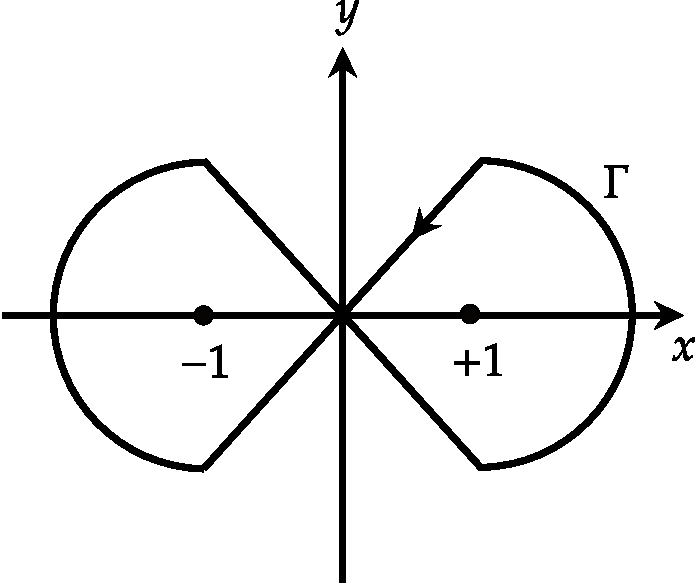
\includegraphics[height=4cm,width=5cm]{diagram-20211005(19)-crop}
	\end{figure}
	\begin{tasks}(4)
		\task[\textbf{A.}] 0
		\task[\textbf{B.}] $2 \pi$
		\task[\textbf{C.}] $-2 \pi$
		\task[\textbf{D.}] $4 \pi i$
	\end{tasks}
	\begin{answer}
		\begin{align*}
		f(z)&=\frac{z e^{i z \pi / 2}}{(z+1)(z-1)}\\
		\text{For }z&=+1\text{ anti-clockwise}\\
		I&=2 \pi i \lim _{z \rightarrow 1} \frac{z e^{i \pi z / 2}}{(z+1)}=\frac{2 \pi i}{2} e^{i \pi / 2}=\pi i e^{i \pi / 2}\\
		\text{For }z&=-1\\
		I&=-2 \pi i \lim _{z \rightarrow-1} \frac{z e^{i \pi z / 2}}{(z-1)}=-2 \pi i \times \frac{(-1) e^{-i \pi / 2}}{(-2)}=-\pi i e^{-i \pi / 2}\\
		\text{Integral }&=\pi i \frac{\left(e^{i \pi / 2}-e^{-i \pi / 2}\right)}{2 i} \times 2 i=2 \pi i^{2} \sin \frac{\pi}{2}=-2 \pi
		\end{align*}
		So the correct answer is \textbf{Option (C)}
	\end{answer}
	\item What is the value of $a$ for which $f(x, y)=2 x+3\left(x^{2}-y^{2}\right)+2 i(3 x y+a y)$ is an analytic function of complex variable $z=x+i y$
	{\exyear{NET/JRF(JUNE-2018)}}
	\begin{tasks}(4)
		\task[\textbf{A.}] 1
		\task[\textbf{B.}] 0
		\task[\textbf{C.}] 3
		\task[\textbf{D.}] 2
	\end{tasks}
	\begin{answer}
		\begin{align*}
		f(x, y)&=2 x+3\left(x^{2}-y^{2}\right)+2 i(3 x y+\alpha y)\\
		u&=2 x+3\left(x^{2}-y^{2}\right), v=2(3 x y+\alpha y)\\
		\text{C-R conditions: }u_{x}&=v_{y}, u_{y}=-v_{x}\\
		2+3(2 x)&=2(3 x+\alpha) \Rightarrow \alpha=1 \Rightarrow-6 y=-6 y
		\end{align*}
		So the correct answer is \textbf{Option (A)}
	\end{answer}
	\item  The value of the integral $\oint_{C} \frac{d z}{z} \frac{\tanh 2 z}{\sin \pi z}$, where $C$ is a circle of radius $\frac{\pi}{2}$, traversed counter-clockwise, with centre at $z=0$, is
	{\exyear{NET/JRF(DEC-2018)}}
	\begin{tasks}(4)
		\task[\textbf{A.}] 4
		\task[\textbf{B.}] $4 i$
		\task[\textbf{C.}] $2 i$
		\task[\textbf{D.}] 0
	\end{tasks}
	\begin{answer}$\left. \right. $
		\begin{figure}[H]
			\centering
			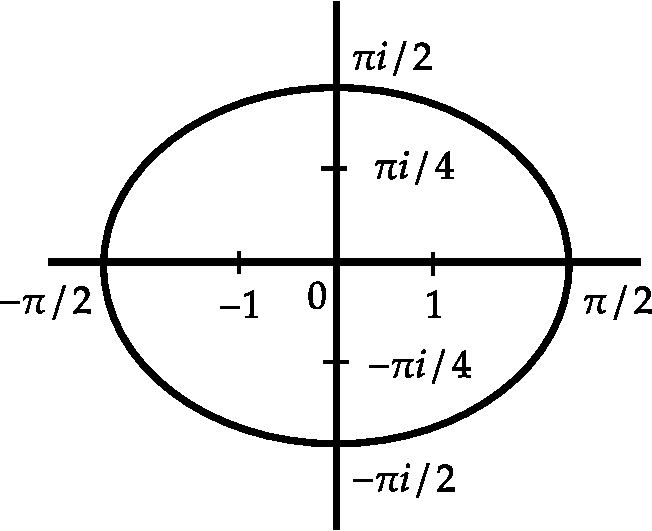
\includegraphics[height=4.5cm,width=5.5cm]{diagram-20211005(2)-crop}
		\end{figure}
		\begin{align*}
		&\oint_{C} \frac{d z}{z} \frac{\tanh 2 z}{\sin \pi z} d z\\
		z&=0,1,-1, \frac{\pi i}{4}, \frac{-\pi i}{4}\\
		f(z)&=\frac{2 z-\frac{1}{3}(2 z)^{3}+\frac{2}{15}(2 z)^{5} \ldots .}{z\left(\pi z-\frac{\pi^{3} z^{3}}{3 !}+\ldots\right)}\\
		\frac{2}{\pi z}&\left(1-\frac{1}{2} z^{2}+\ldots\right)\left(1-\frac{\pi^{2} z^{2}}{2 !}+\ldots\right)\\
		b_{1}&=\frac{2}{\pi}\\
		\text{As Re } z&=1, \frac{\tanh ^{2}}{-\pi}\text{ and }\operatorname{Re} z=-1, \frac{\tanh ^{2}}{-\pi}\\
		\operatorname{Re} z&=\frac{i \pi}{4}=-\frac{1}{\pi}\left(2 \operatorname{cosec} h \frac{\pi^{2}}{4}\right)\\
		\operatorname{Re} z&=\frac{-i \pi}{4}=-\frac{1}{\pi}\left(2 \operatorname{cosec} \mathrm{h} \frac{\pi^{2}}{4}\right)
		\intertext{$I=2 \pi i \Sigma R=4 i$ only when 0 lies inside, otherwise wrong question.}
		\end{align*}
		So the correct answer is \textbf{Option (B)}
	\end{answer}
	\item The integral $I=\int_{C} e^{z} d z$ is evaluated from the point $(-1,0)$ to $(1,0)$ along the contour $C$, which is an arc of the parabola $y=x^{2}-1$, as shown in the figure. The value of $I$ is
	{\exyear{NET/JRF(DEC-2018)}}
	\begin{figure}[H]
		\centering
		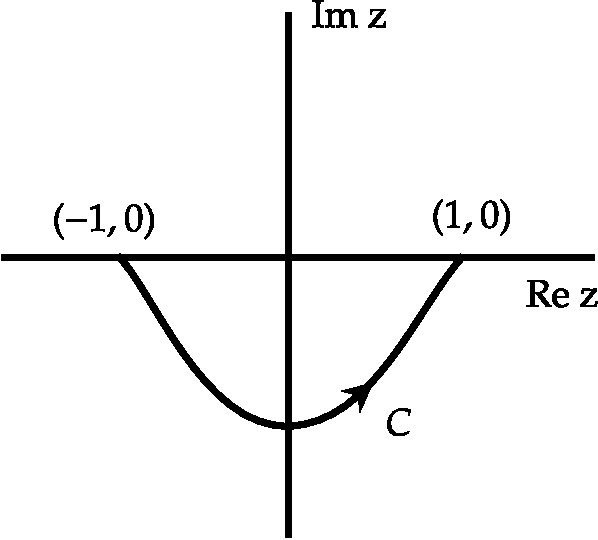
\includegraphics[height=4.5cm,width=5cm]{diagram-20211005(3)-crop}
	\end{figure}
	\begin{tasks}(4)
		\task[\textbf{A.}]  0
		\task[\textbf{B.}] $2 \sinh 1$
		\task[\textbf{C.}]  $e^{2 i} \sinh 1$
		\task[\textbf{D.}] $e+e^{-1}$
	\end{tasks}
	\begin{answer}
		\begin{align*}
		\int_{C} f(z) d z&=2 \pi i \Sigma R\\
		\int_{C} f(z) d z+\int_{1}^{-1} e^{x} d x&=0\\
		\int_{C} f(z) d z&=-\int_{1}^{-1} e^{x} d x=\int_{1}^{-1} e^{x} d x\\&=\frac{\left(e^{1}-e^{-1}\right)}{2} \cdot 2=2 \sinh 1
		\end{align*}
		So the correct answer is \textbf{Option (B)}
	\end{answer}
	\item The contour $C$ of the following integral
	$$
	\oint_{C} d z \frac{\sqrt{(z-1)(z-3)}}{\left(z^{2}-25\right)^{3}}
	$$
	in the complex $z$ plane is shown in the figure below.\\
	\begin{figure}[H]
		\centering
		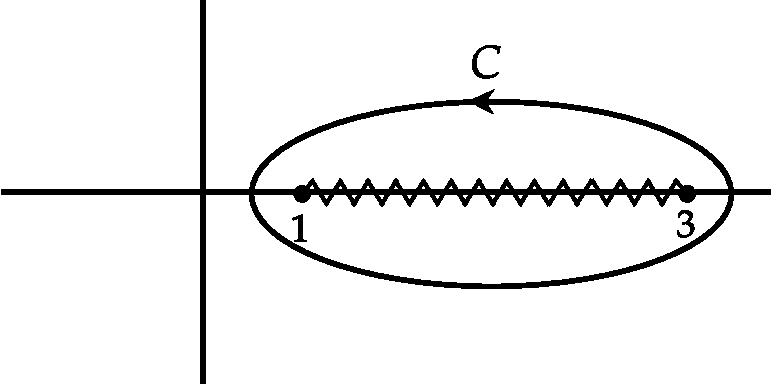
\includegraphics[height=3.5cm,width=6cm]{diagram-20211005(8)-crop}
	\end{figure}
	This integral is equivalent to an integral along the contours
	{\exyear{NET/JRF(DEC-2018)}}
	\begin{tasks}(2)
		\task[\textbf{A.}] \begin{figure}[H]
			\centering
			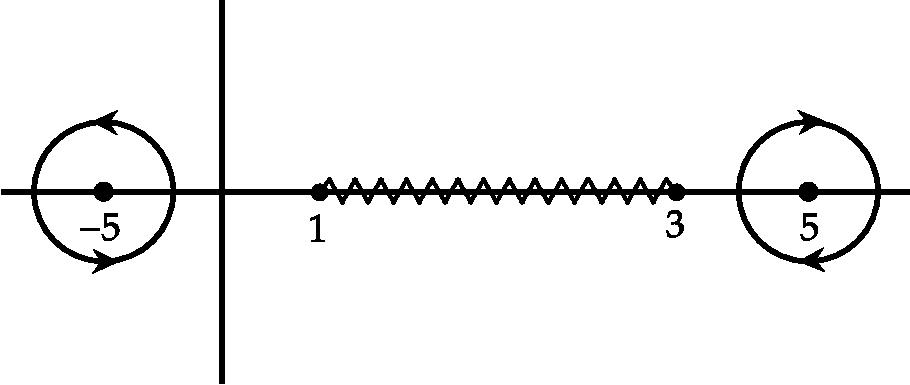
\includegraphics[height=3cm,width=6.5cm]{diagram-20211005(4)-crop}
		\end{figure}
		\task[\textbf{B.}] \begin{figure}[H]
			\centering
			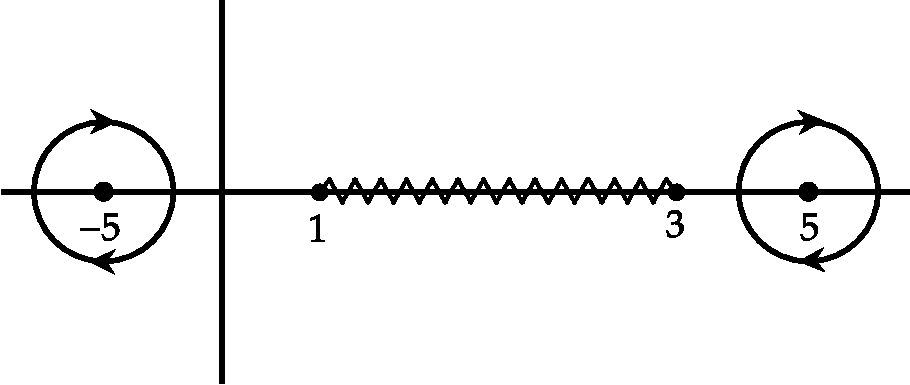
\includegraphics[height=3cm,width=6.5cm]{diagram-20211005(5)-crop}
		\end{figure}
		\task[\textbf{C.}] \begin{figure}[H]
			\centering
			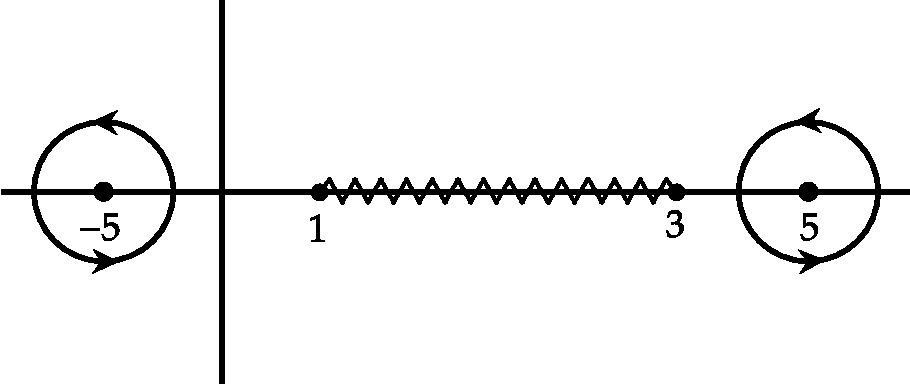
\includegraphics[height=3cm,width=6.5cm]{diagram-20211005(6)-crop}
		\end{figure}
		\task[\textbf{D.}] \begin{figure}[H]
			\centering
			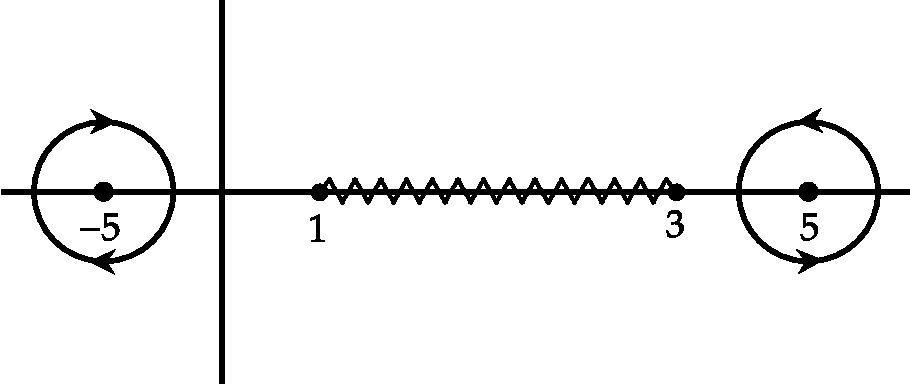
\includegraphics[height=3cm,width=6.5cm]{diagram-20211005(7)-crop}
		\end{figure}
	\end{tasks}
	\begin{answer}
		\begin{align*}
		\intertext{$z=1,3$ are branch points $\infty$ is not a branch point 1 branch cut 3}
		\end{align*}
		So the correct answer is \textbf{Option (C)}
	\end{answer}
	\item  Let $C$ be the circle of radius $\frac{\pi}{4}$ centered at $z=\frac{1}{4}$ in the complex $z$-plane that is traversed counter-clockwise. The value of the contour integral $\oint_{C} \frac{z^{2}}{\sin ^{2} 4 z} d z$ is
	{\exyear{NET/JRF(DEC-2019)}}
	\begin{tasks}(4)
		\task[\textbf{A.}] 0
		\task[\textbf{B.}] $\frac{i \pi^{2}}{4}$
		\task[\textbf{C.}] $\frac{i \pi^{2}}{16}$
		\task[\textbf{D.}] $\frac{i \pi}{4}$
	\end{tasks}
	\begin{answer}$\left. \right. $
		\begin{figure}[H]
			\centering
			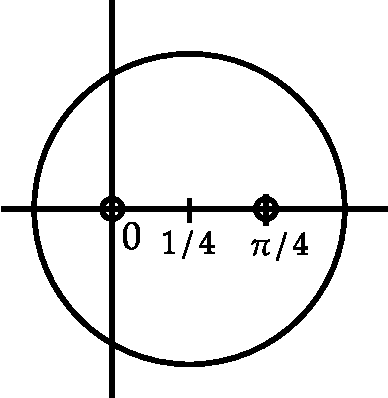
\includegraphics[height=3cm,width=3cm]{diagram-20211026(16)-crop}
		\end{figure}
		\begin{align*}
		f(z)&=\left(\frac{\pi}{\sin 4 z}\right)^{2}\\
		z_{0}&=0, \frac{\pi}{4}\text{ are poles}\\
		4 z&=n \pi, z=0, \frac{\pi}{4}
		\intertext{Others are outside the contour.}
		\text{Residue at }z&=0\text{ is }\left[\frac{\pi}{4 z-\frac{4^{3} z^{3}}{3 !}+\ldots}\right]^{2}\\
		&=\left[\frac{1}{4-\frac{4^{3} z^{2}}{3 !}+\ldots .}\right]^{2}\qquad \text{ No terms for } \frac{1}{z}, b_{1}=0\\
		&=\left[4-\frac{4^{3} z^{2}}{3 !}+\ldots .\right]^{-2}\\
		\text{Residue for }z&=\frac{\pi}{4}\\
		z-\frac{\pi}{4}&=t
		\intertext{$\sin (4 t+\pi)=-\sin 4 t \quad$ (But square so no effect)}
		&\left[\frac{t+\frac{\pi}{4}}{\sin 4\left(t+\frac{\pi}{4}\right)}\right]^{2}\\
		\left(\frac{t+\frac{\pi}{4}}{\sin 4 t}\right)^{2}&=\frac{t^{2}+\frac{\pi^{2}}{4}+2 t \cdot \frac{\pi}{4}}{\sin ^{2} 4 t}\\
		\frac{\pi}{2} \frac{t}{16 t^{2}[1-\ldots .]^{2}}&=\frac{\pi}{32 t}[1-\ldots .]^{-2} \text{(from first term)}\\
		b_{1}&=\frac{\pi}{32}\\
		\oint_{C} \frac{z^{2}}{\sin ^{2} 4 z} d z&=2 \pi i\left[0+\frac{\pi}{32}\right]=\frac{i \pi^{2}}{16}
		\end{align*}
		So the correct answer is \textbf{Option (C)}
	\end{answer}
	\item  A function of a complex variable $z$ is defined by the integral $f(z)=\oint_{\Gamma} \frac{w^{2}-2}{w-z} d w$, where $\Gamma$ is a circular contour of radius 3 , centred at origin, running counter-clockwise in the $w$ - plane. The value of the function at $z=(2-i)$ is
	{\exyear{NET/JRF(JUNE-2020)}}
	\begin{tasks}(4)
		\task[\textbf{A.}] 0
		\task[\textbf{B.}] $1-4 i$
		\task[\textbf{C.}]  $8 \pi+2 \pi \mathrm{i}$
		\task[\textbf{D.}] $-\frac{2}{\pi}-\frac{i}{2 \pi}$
	\end{tasks}
	\begin{answer}$\left. \right. $
		\begin{figure}[H]
			\centering
			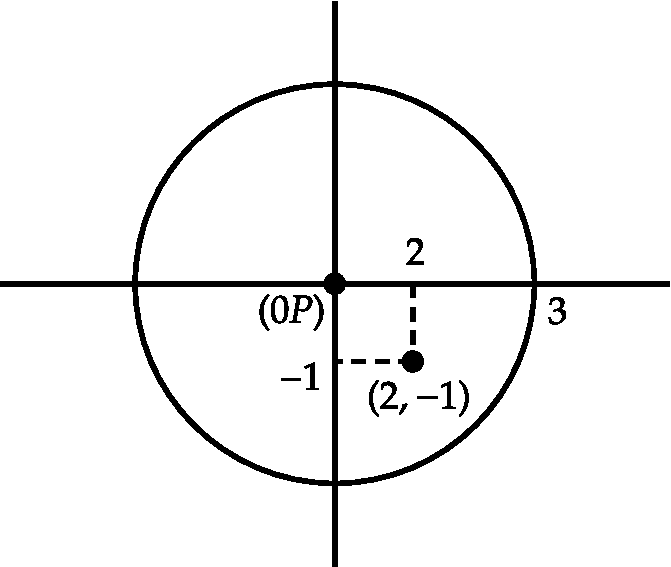
\includegraphics[height=4cm,width=4.6cm]{diagram-20211027-crop}
		\end{figure}
		\begin{align*}
		f(z)&=\oint_{\Gamma} \frac{w^{2}-2}{w-z} d w\\
		\omega&=z\text{ is a simple pole.}\\
		\text{Residue }\lim _{\omega \rightarrow z}(\omega-z) \frac{\left(\omega^{2}-2\right)}{(\omega-z)}&=(2-i)^{2}-2 \\&=4-1-4 i-2=(1-4 i)\\
		f(z)&=\oint_{\Gamma} \frac{w^{2}-2}{w-z} d w=2 \pi i(1-4 i)=2 \pi i+8 \pi
		\end{align*}
		So the correct answer is \textbf{Option (C)}
	\end{answer}
\end{enumerate}
\colorlet{ocre1}{ocre!70!}
\colorlet{ocrel}{ocre!30!}
\setlength\arrayrulewidth{1pt}
\begin{table}[H]
	\centering
	\arrayrulecolor{ocre}
	\begin{tabular}{|p{1.5cm}|p{1.5cm}||p{1.5cm}|p{1.5cm}|}
		\hline
		\multicolumn{4}{|c|}{\textbf{Answer key}}\\\hline\hline
		\rowcolor{ocrel}Q.No.&Answer&Q.No.&Answer\\\hline
		1&\textbf{C} &2&\textbf{B}\\\hline 
		3&\textbf{B} &4&\textbf{A} \\\hline
		5&\textbf{A} &6&\textbf{D} \\\hline
		7&\textbf{A}&8&\textbf{-}\\\hline
		9&\textbf{C}&10&\textbf{A}\\\hline
		11&\textbf{C} &12&\textbf{-}\\\hline
		13&\textbf{A}&14&\textbf{B}\\\hline
		15&\textbf{C}&16&\textbf{B}\\\hline
		17&\textbf{C} &18&\textbf{A}\\\hline
		19&\textbf{B}&20&\textbf{B}\\\hline
		21&\textbf{C}&22&\textbf{C}\\\hline
		23&\textbf{C}& &\\\hline
		
	\end{tabular}
\end{table}